\chapter{Requirements and Design}

%The bulk of the design and implementation of an interactive interface to the MS-PROD model has been completed.  However, this is not a final design; in many cases, several design alternatives have been implemented and await the evaluation study prior to final implementation.  These alternatives are described below.

The motivation of this research is to provide an interactive interface to the NOAA MS-PROD model so as to help fishermen, fisheries managers, and other stakeholders understand the implications of decisions, such as changing catch quotas for particular kinds of fishing activity---e.g., bottom trawling versus mid-water trawling.  We planned our interactive interface with the intent that users would gain insight into:

\begin{itemize}
	\item \textbf{Implications of the model:}  E.g., how do two different sets of fishing effort values affect the biomass predictions of the ten species?
	\item \textbf{The model itself:}  E.g., why does the abundance of one species increase when another species is caught? 
\end{itemize} 

To accomplish this goal, we determined our interactive interface of the MS-PROD model would need to visualize:

\begin{itemize}
	\item The predicted biomass over time,
	\item Changes in predicted biomass as a result of changes in fishing effort,
	\item Causal relationships which help to explain indirect or unintuitive results,
	\item Uncertainty of the model
\end{itemize} 

Since setting fishing quotas is the only action fishery managers can take, we determined that the only interaction available to users would be to adjust the fishing effort level; all other model parameters are not modifiable while the model and its visualization are running.  This interaction is done by means of a set of sliders with the goal of allowing the user to immediately see the impact of management decisions on fisheries.  The user adjusts sliders which represent harvest effort and watches the biomass plots change instantaneously as the model is re-run according to the new effort values.  Like Eberlein and Peterson, we aimed to turn the ``time consuming and tedious'' task of working with a model into a ``fast and fun'' interactive experience \cite{eberlein1992}.  Different views and features of the model visualization are described and discussed in the sections below.  

It is important to note that the MS-PROD model allows for different fishing effort values for each species for each year in the thirty-year period that the model produces forecasts for.  This is to reflect that fishing quotas can change from year to year.  Since there are ten species and thirty years, this means there are potentially 300 separate fishing effort values that could be set by a user.  However, it would be cluttered and confusing to have an effort slider for each of those 300 values.  Therefore, two simplifications were made.  First, fishing effort should be controlled by functional group rather than individual; the model authors requested this because it is more realistic than fishing by individual species.  Second, fishing effort for a functional group is constant across all thirty years; while this is unrealistic, it is easier to understand and perhaps, in a sustainable, ``perfect world,'' fishing quotas would not need adjusting over the years.  Thus, each slider controls the fishing effort for all thirty years for a particular functional group.

\section{Visualization of Predicted Biomass}

First and foremost, we had to decide how to display the thirty-year biomass forecast data output by the model.  Time series line charts---of both the simple line chart and small multiples varieties---were chosen because casual viewers can understand them without further instructions, as opposed to, say a horizon graph.  Another advantage to line charts is that they tend to have a reasonable amount of whitespace where additional information can be displayed, such as uncertainty or alternate forecasts. A key design issue concerned the representation of change; line charts provide the ability to display this change.  A number of alternatives for change were implemented and are described in the sections that follow.

\subsection{Alternative Screen Layouts}

Once it was decided that time series were most appropriate for our task, we had to choose how many individual charts should be used to display the data and how to arrange them.  Two alternative screen layouts were developed for displaying these time series on line charts: a ``four panel'' view in Figure~\ref{fig:msprod_group} and a ``small multiple'' view in Figure~\ref{fig:msprod_species}, described in further detail below.  With both views, the time series for the species are organized by functional group.  A functional group is a biological grouping of species which perform similar functions within their ecosystem---e.g., mackerel and herring are both members of the ``small pelagic'' group since they live in the water column.

There were several reasons for the decision to arrange by functional group rather than placing all time series on a single line chart.  First, harvest effort is controlled by functional group using the sliders, so it must be somehow indicated which species are part of which functional group.  With multiple time series, this can be encoded through positioning by arranging the slider of a functional group to be near the time series of that group's species.  Second, it would have been impractical to simply place all time series on a single line chart because would have been difficult to select enough distinct colors to represent each of the ten species.  Furthermore, the biomass of some species is significantly larger than others.  By scaling the $y$-axis according to the largest biomass value of all species in the entire 30-year time span, the lines representing some species would have been crowded at the bottom of the chart and seemed to be flat even when they were not.

\subsubsection{Four Panel View}

\begin{figure}[h]
	\centering
	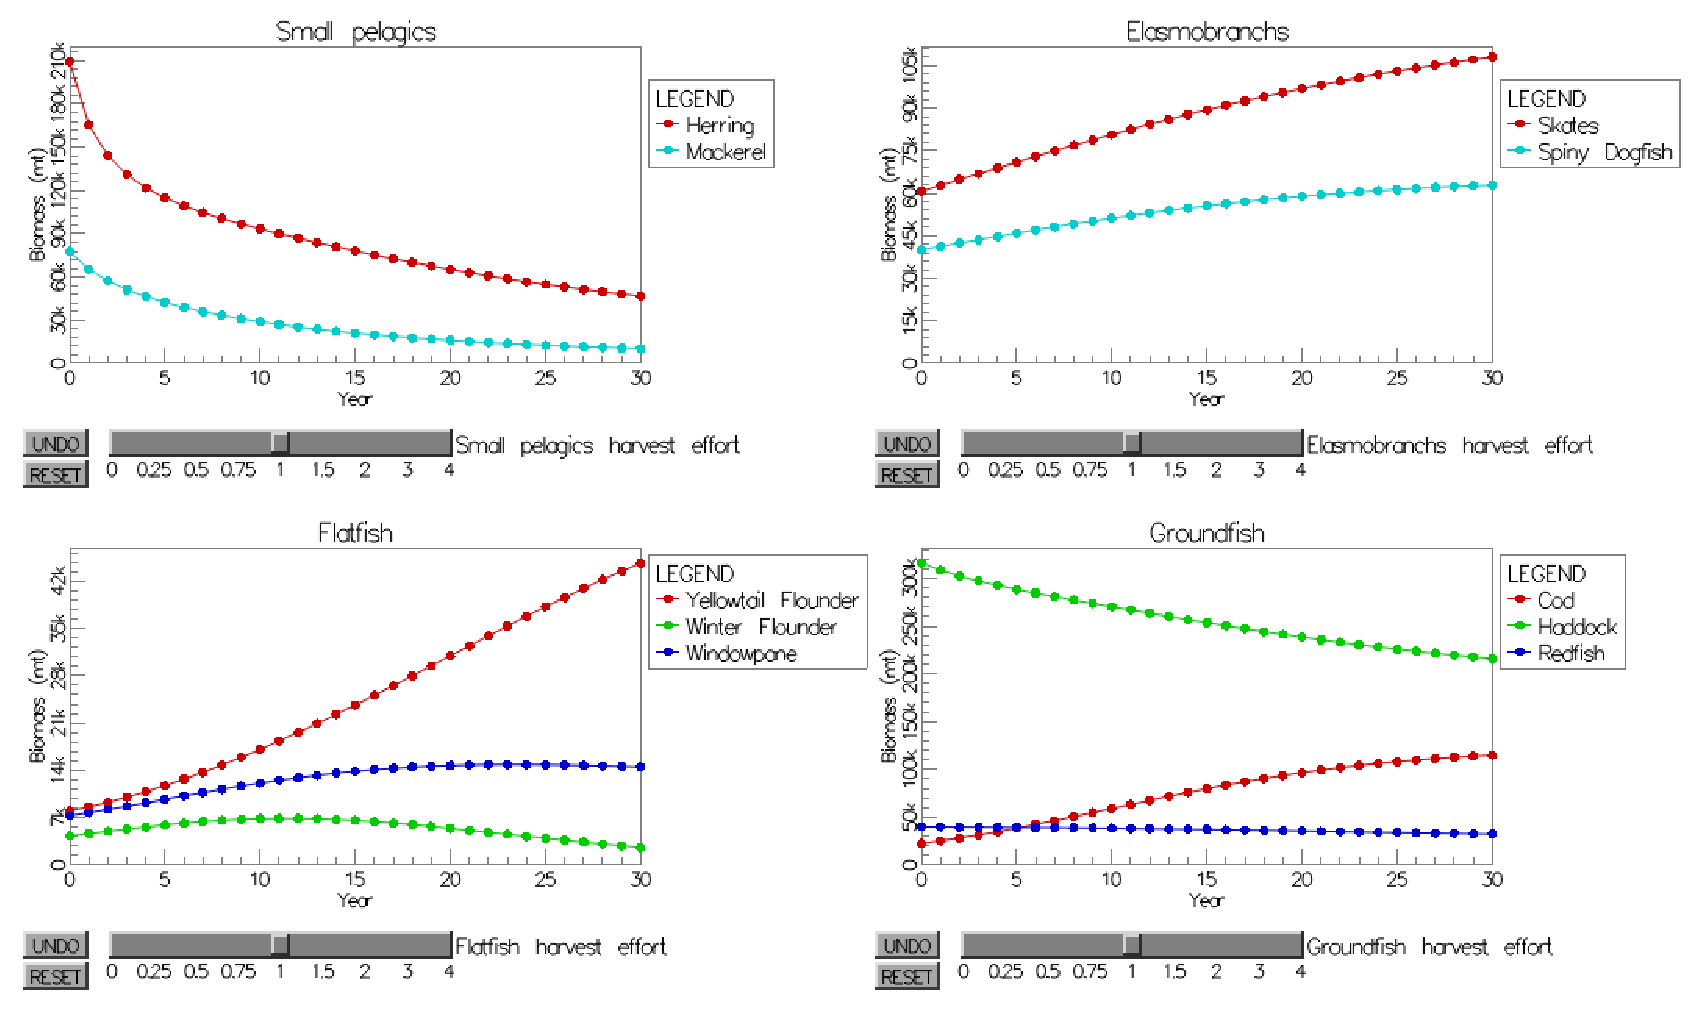
\includegraphics[width=14cm]{figures/eps/msprod_group.eps}
	\caption{The ``four panel'' view of our MS-PROD visualization.}
	\label{fig:msprod_group}
\end{figure}

It was observed that species of similar functional groups tend to have biomass values in similar numeric ranges, so a decision was made to make one line chart per functional group for displaying biomasses.  This view is called the ``four panel'' view and is shown in Figure~\ref{fig:msprod_group}.

The major advantage of this ``four panel'' view is that comparisons of species within a group are easy.  For MS-PROD, there are only two or three species per functional group, so the line chart for each group tends to not suffer from occlusion problems.  Direct and indirect effects of changes in harvest effort are easily differentiated with the ``four panel'' approach---e.g., if the user adjusts the effort slider only for elasmobranchs, yet sees the biomasses change on the groundfish chart, then the user can begin to understand there is some kind of relationship between elasmobranchs and groundfish.

\subsubsection{Small Multiples View}

\begin{figure}[h]
	\centering
	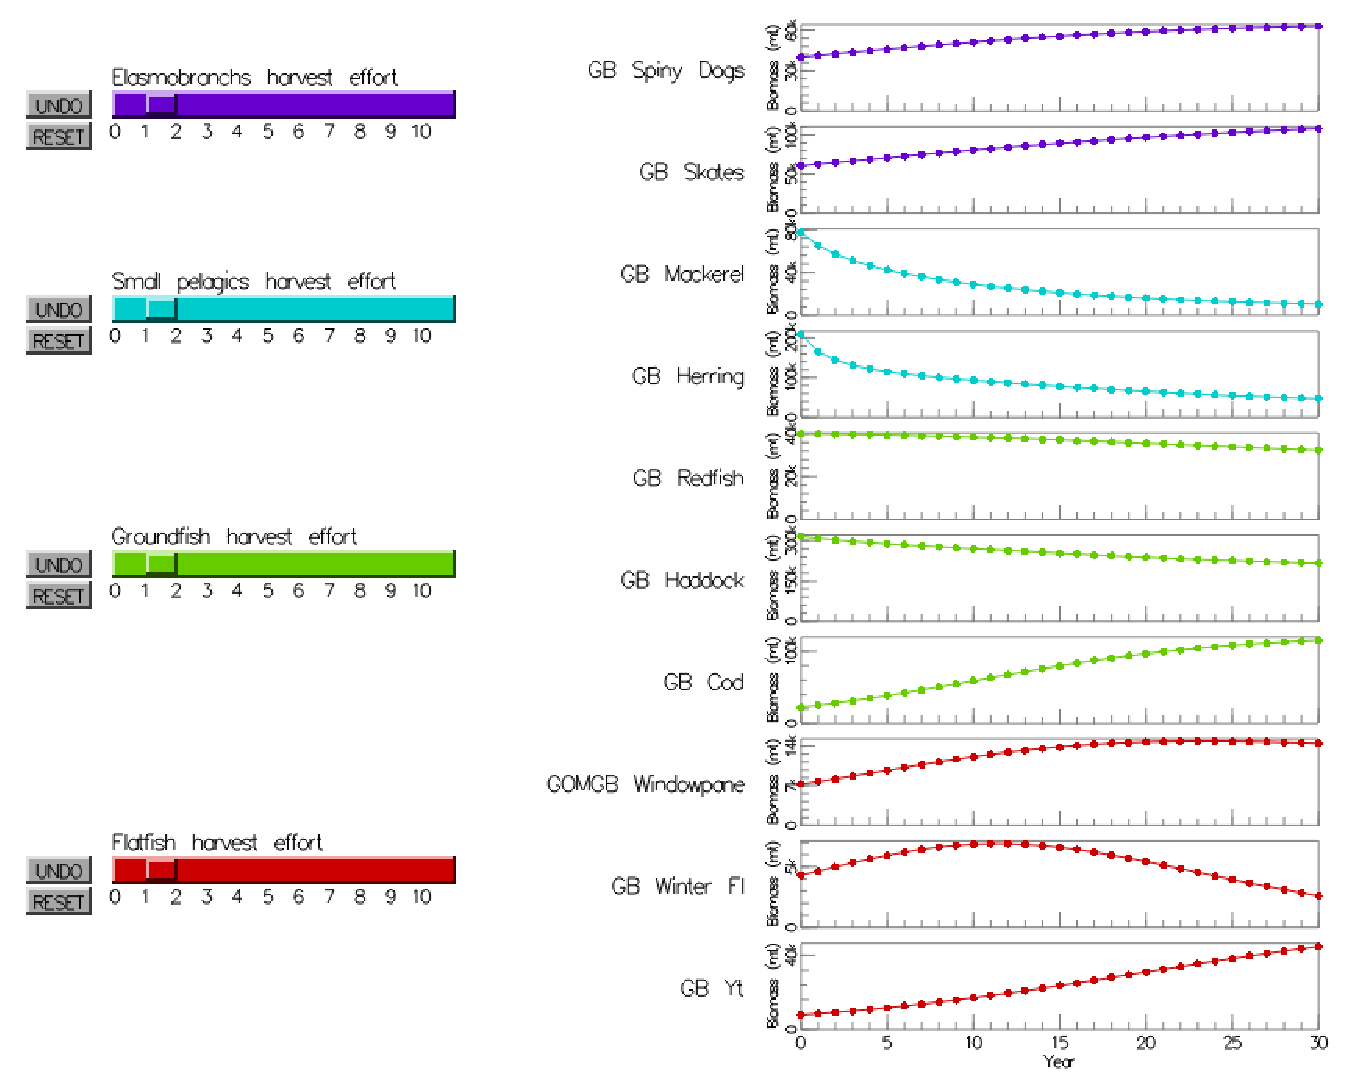
\includegraphics[width=12cm]{figures/eps/msprod_species.eps}
	\caption{The ``small multiples'' view of our MS-PROD visualization.}
	\label{fig:msprod_species}
\end{figure}

The alternative to the ``four panel'' view is to view each species on its own plot, which we call the ``small multiple'' view.  The main purpose of this view was to support the addition of arc graph connections between species, as are discussed later in Section~\ref{sec:arc}. Shown in Figure~\ref{fig:msprod_species}, each plot is sorted and colored according to functional group membership, using Cleveland's recommendations for chart size \cite{cleveland1988}.  The harvest effort sliders are also colored by functional group and positioned near the plots of the corresponding group.  This allows for the ability to differentiate between direct and indirect effects of changes in harvest effort.

With each species on its own plot, it is much easier to interpret the biomass predictions of an individual species, since the $y$-dimension of a plot needs to be scaled to the data of one species only.  It is easier to perceive increases or decreases in biomass because no species suffer from the ``flattening'' that can occur when a series is displayed on the same plot as a series that has significantly higher values.  On the other hand, this makes biomass comparison between species somewhat difficult because the user must either refer to the $y$-axis labels or hover over a specific point on a chart, which causes a label to appear, in order to determine the absolute value of the biomass at a point in time.

\subsubsection{Absolute Biomass Indicators}

\begin{figure}[h]
	\centering
	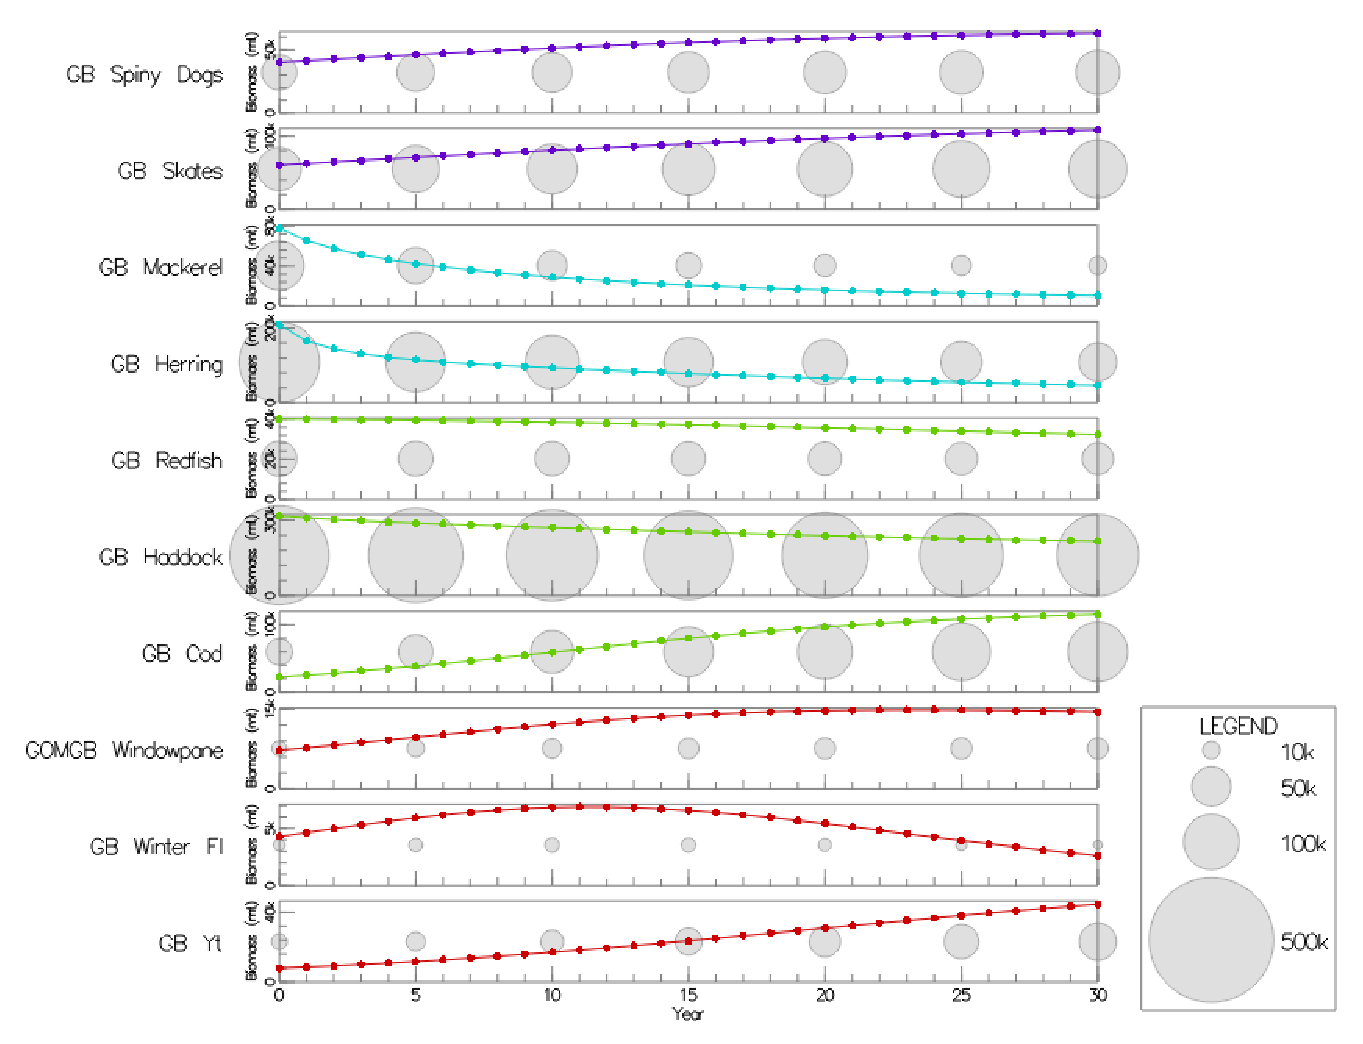
\includegraphics[width=11cm]{figures/eps/msprod_abssize.eps}
	\caption{Absolute biomass indicators overlaying the ``small multiples'' view.}
	\label{fig:msprod_abssize}
\end{figure}

Absolute biomass indicators, seen in Figure~\ref{fig:msprod_abssize}, were introduced to show how biomass changes over time by showing the absolute biomass of the population as the area of a circle.  This makes comparison across species possible.  To avoid occlusion, these indicators are drawn every five years within the thirty-year time span.

\section{Visualization of Change}

\begin{figure}
\centering
	\begin{subfigure}[b]{0.8\textwidth}
		\centering
		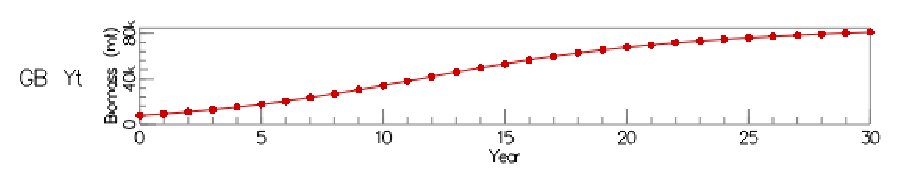
\includegraphics[width=11cm]{figures/eps/msprod_change_none.eps}
		\caption{Change shown by interaction.}	
		\label{fig:changeNone}
	\end{subfigure}	\\
	\begin{subfigure}[b]{0.8\textwidth}
		\centering
		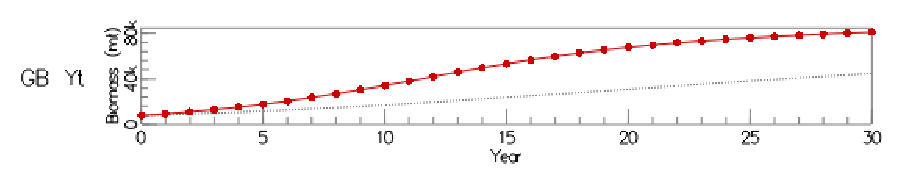
\includegraphics[width=11cm]{figures/eps/msprod_change_line.eps}
		\caption{The status quo is shown as the dotted gray line.}
		\label{fig:changeLine}
	\end{subfigure} \\
	\begin{subfigure}[b]{0.8\textwidth}
		\centering
		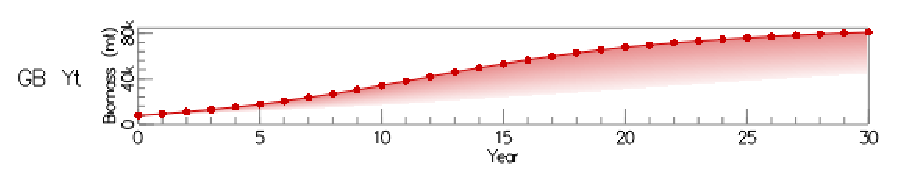
\includegraphics[width=11cm]{figures/eps/msprod_change_blend.eps}
		\caption{The area between the status quo graph and the new forecast is shaded.}
		\label{fig:changeBlend}
	\end{subfigure}
	\caption{The three options for depicting change between current biomass predictions and baseline predictions.}
	\label{fig:changeTypes}
\end{figure}

In order for modelers and other stakeholders to understand and compare decisions, the ability to perceive changes in biomass resulting from changes in the fishing effort is required.  Therefore, we have introduced a feature that allows the user to compare the forecast effects of a change in fishing effort compared to the forecasts of the \textit{status quo} [baseline]. There are three alternatives for displaying forecast differences with the baseline.  The first is to simply have the biomass plots change instantaneously as the harvest effort sliders are adjusted, as in Figure~\ref{fig:changeNone}.  The second is a dotted gray line which shows the forecast of the baseline in addition to the current forecast, shown in Figure~\ref{fig:changeLine}.  The third is a shaded area originating from the curve of the current forecast that diminishes in opacity as it approaches the curve of the baseline forecast, as in Figure~\ref{fig:changeBlend}.

\begin{figure}[h]
	\centering
	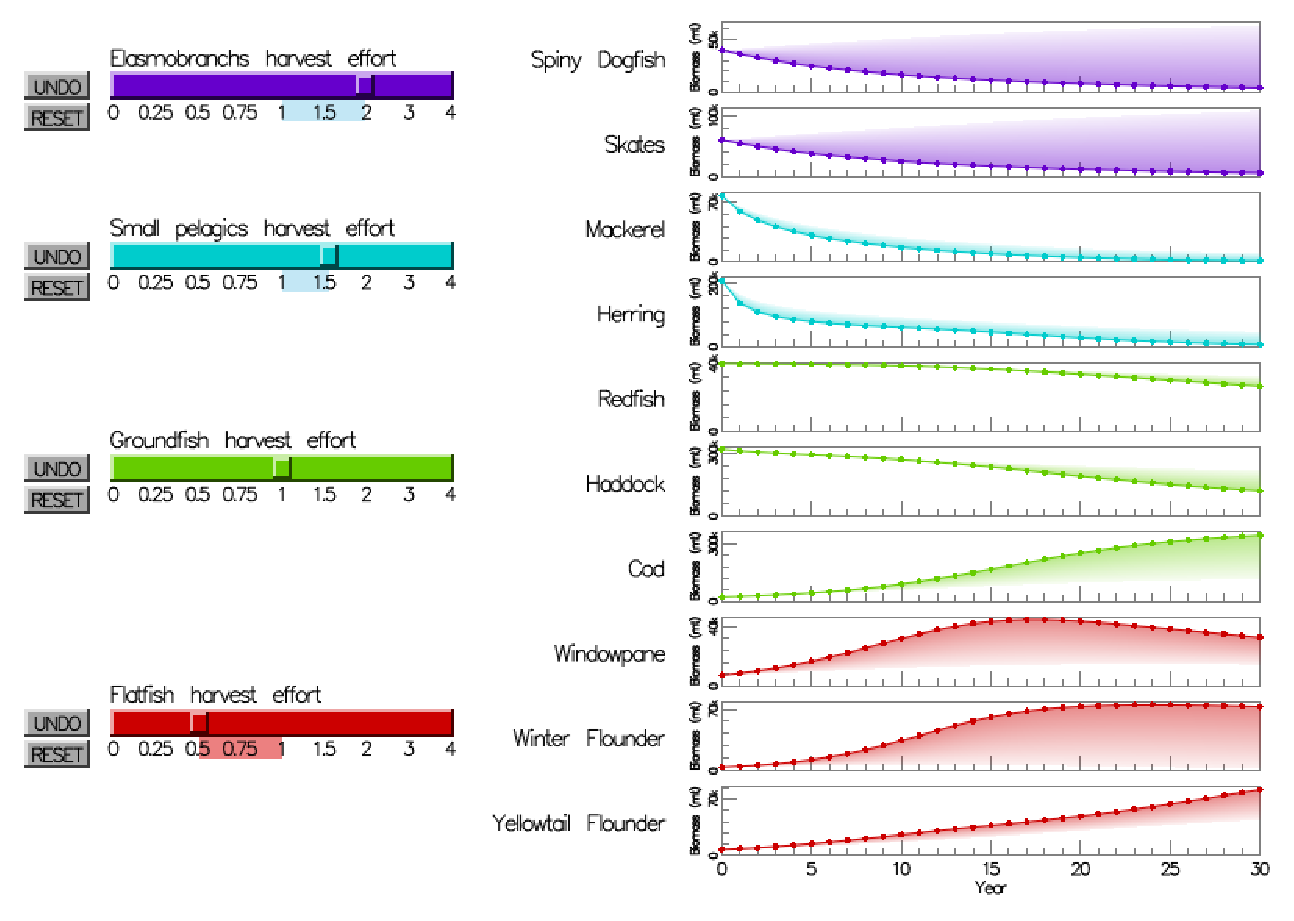
\includegraphics[width=12cm]{figures/eps/msprod_change.eps}
	\caption{Showing change between different effort values.}
	\label{fig:msprod_change}
\end{figure}

Figure~\ref{fig:msprod_change} shows all of the time series in the ``small multiples'' view with the effort sliders and the blended change option enabled.  Again, the blended area in a line chart is colored from the current biomass line to the line as it was when the baseline was set; a colored area above the line indicates the biomass declined, while a colored area beneath represents the biomass increased---e.g., the ``skate'' population declined dramatically with the new effort values, the ``winter flounder'' population increased due to the changes, and ``haddock'' seemed to be unaffected.

Underneath each slider, a colored rectangle---if present---indicates differences from the baseline effort settings.  Blue indicates the effort value has been increased since the baseline was set---e.g., again in Figure~\ref{fig:msprod_change}, the effort for ``elasmobranchs'' was originally set to 1.0 and now it is approximately 2.0.  Red represents the effort value has been decreased since the baseline was set---e.g., the effort for ``flatfish'' was originally set to 1.0 and now it is approximately 0.5.

This feature is available in both the ``four panel'' and ``small multiples'' views.  The baseline effort setting can be defined at any time with a simple button at the top of the screen.  This resets the baseline as the current slider settings.  Buttons are also available to undo or reset changes to the effort values.

\section{Visualization of Causal Relationships}
%\label{sec:arc}

Understanding of the model requires understanding of the underlying relationships between species---namely, \textit{predation} and \textit{competition}---and \textit{harvest}.  As defined earlier, predation is when one species consumes another and competition accounts for any way species might impact another in a way that is not predation.  Harvest is process of humans trying to catch fish in the wild.  Our interface must explain to users which species impact each other, how harvesting impacts the species, and the magnitude of those relationships.  These relationships are illustrated by a node-link diagram, where the nodes are the time series of the fish species and the harvest effort sliders.

\subsection{Inter-Species Relationships}

\begin{figure}
\centering
	\begin{subfigure}[b]{0.33\textwidth}
		\centering
		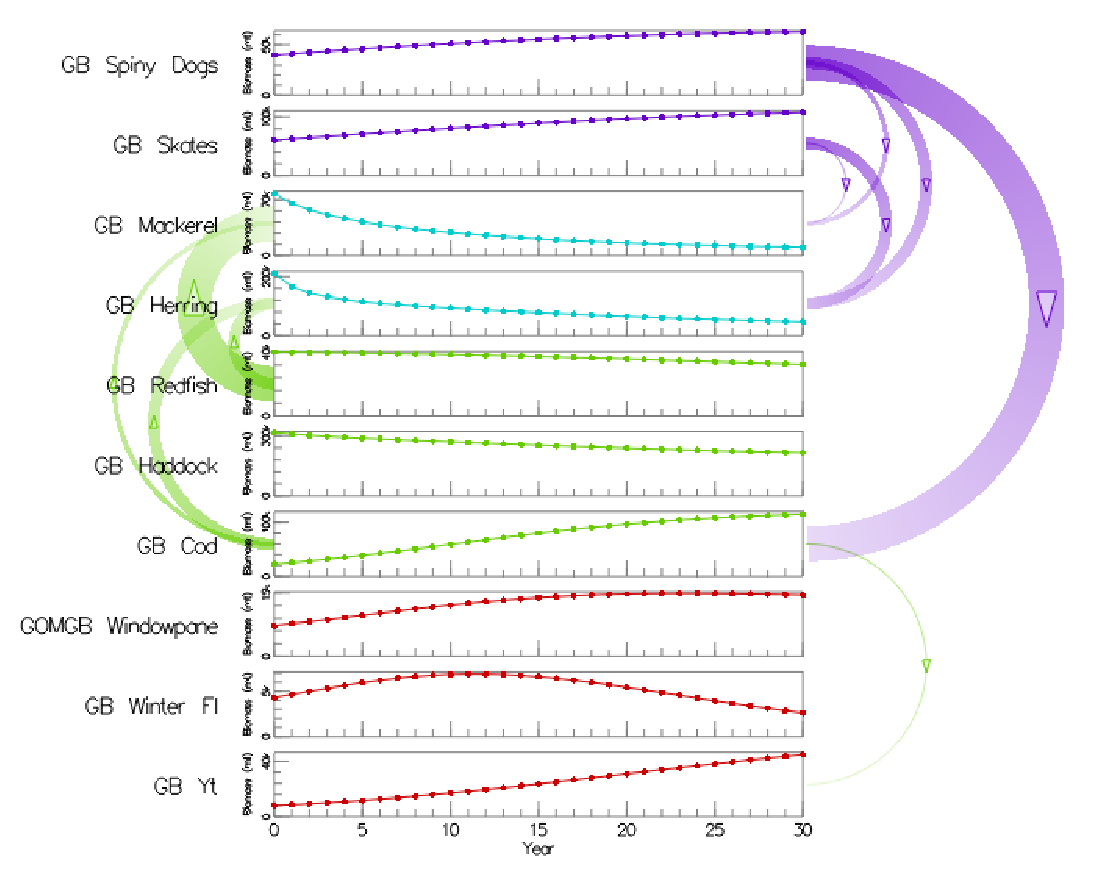
\includegraphics[width=1\textwidth]{figures/eps/arcs_predation.eps}
		\caption{Predation arcs.}
		\label{fig:arcsPredation}
	\end{subfigure}	
	\begin{subfigure}[b]{0.33\textwidth}
		\centering
		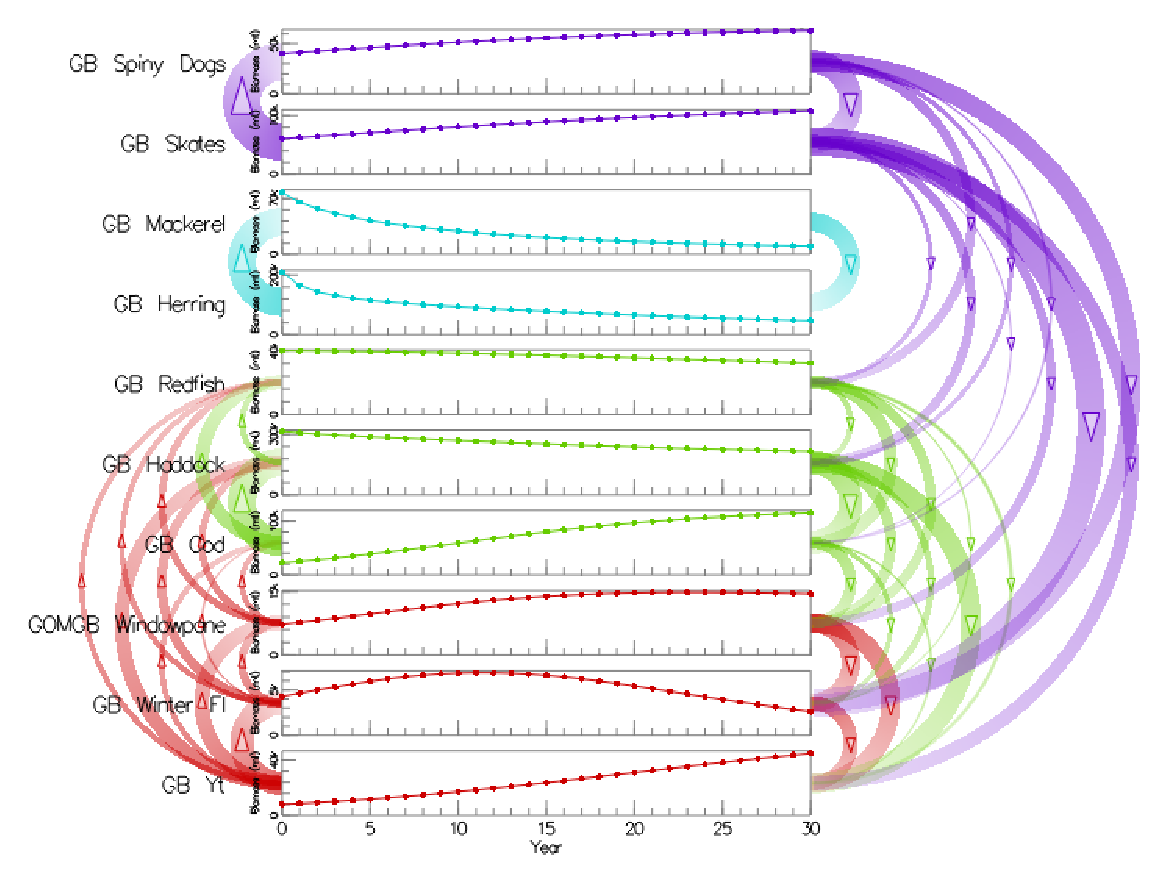
\includegraphics[width=1\textwidth]{figures/eps/arcs_interaction.eps}
		\caption{Competition arcs.}
		\label{fig:arcsCompetition}
	\end{subfigure}
	\begin{subfigure}[b]{0.32\textwidth}
		\centering
		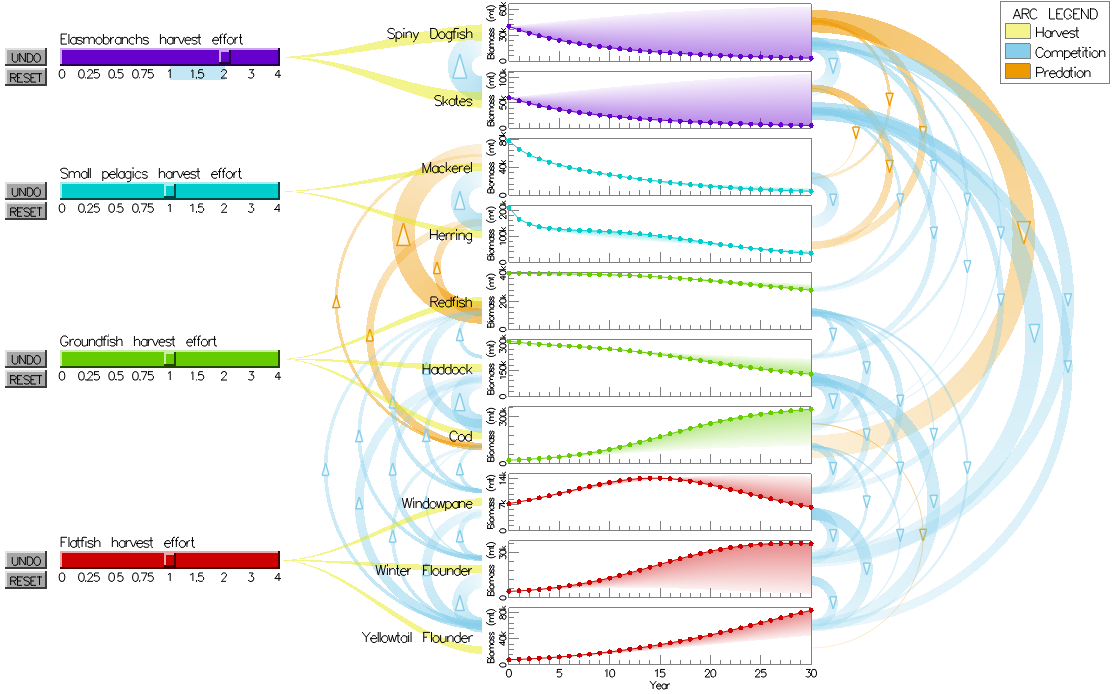
\includegraphics[width=1\textwidth]{figures/eps/arcs_static.eps}
		\caption{Both types of arcs.}
		\label{fig:arcsBoth}
	\end{subfigure}
	\caption{Static arcs drawn between species charts to represent relationships.}
	\label{fig:betweenSpeciesArcs}
\end{figure}

The inter-species relationships are illustrated with arc diagram network visualizations between time series, as in Figure~\ref{fig:betweenSpeciesArcs}.  In the input parameter file, predation and competition coefficient matrices are defined to represent the relationship between each pair of species.  Each non-zero coefficient is represented with an arc connecting the time series plots of the corresponding species.  This is only available in the small multiples view because there are multiple species represented in each plot of the four panel view.

The arc diagram was selected over other network visualizations because it is easily combined with the small multiples.  A separate node-link diagram, such as one with a force-directed layout, may have been confusing because it would require the user to mentally associate nodes in the network with line charts.  An arc diagram does not suffer from this problem since, in our case, the time series themselves are the nodes.  Furthermore, the arc diagram enhances the entire visualization without occluding the time series.  Arc diagrams are also well suited to smaller datasets with clusters of nodes, which applies to our dataset since the fish are segmented into functional groups.

\subsubsection{Directionality}

\begin{figure}[h]
	\centering
	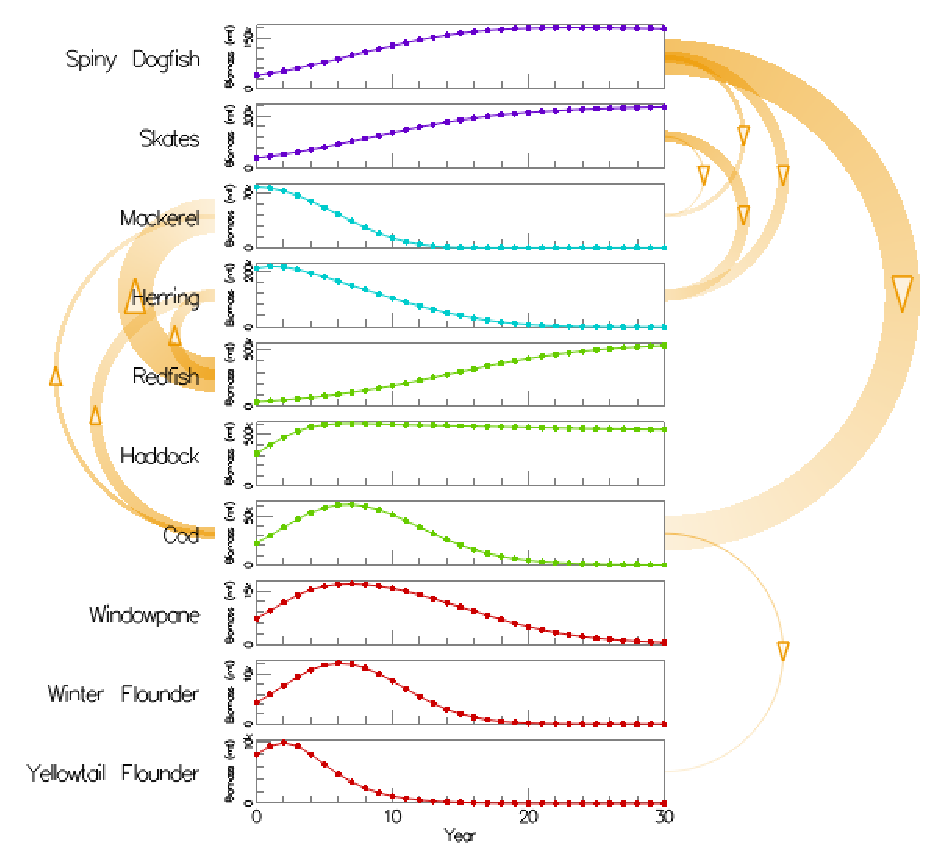
\includegraphics[width=0.85\textwidth]{figures/eps/arcs_directionality.eps}
	\caption{Static predation arcs with directionality indicated by a triangular arrow, fading color intensity, and clockwise direction.}
	\label{fig:arcs_directionality}
\end{figure}

These relationships, predation and competition, both imply directionality, where one species of fish is the ``source'' and the other species is the ``recipient.''  Therefore, our arcs have been drawn with fading opacity to indicate the direction, since Holten and van Wijk recommended a dark-to-light representation for an intensity-based cue \cite{holten2009}.  Additionally, our arcs follow a clockwise direction.  This is necessary because there may be reciprocal ``Fish A affects Fish B'' and ``Fish B affects Fish A'' relationships, especially for the competition type of relationship, so arcs must be drawn on both sides of the time series, as seen in Figure~\ref{fig:betweenSpeciesArcs}.  Additionally, triangular marks have been drawn in the middle of the arcs to point from the originator to the recipient species.  These three directionality cues can be seen in Figure~\ref{fig:arcs_directionality}.

\subsubsection{Arc Type}

The interface provides a few options for viewing the inter-species relationships.  Firstly, users have the ability to view either predation as in Figure~\ref{fig:arcsPredation}, competition as in Figure~\ref{fig:arcsCompetition}, or both.  Secondly, the arcs can be viewed statically, dynamically without animation, or dynamically with animation; these three arc types are described below.  Regardless of the selected arc type, all predation arcs are colored orange and all competition arcs are colored sky-blue.

\paragraph{Static}

With the static style of the arcs, all arcs are drawn at all times, as shown in all three subfigures of Figure~\ref{fig:betweenSpeciesArcs}.  The width of an arc corresponds to the magnitude of the relationship, as defined in the predation coefficient matrix or the competition coefficient matrix in the original parameter file.  The user can mouse over a particular arc, which causes that arc to highlight while the other arcs fade and displays a label which spells out the relationship in words and shows the original coefficient---e.g., ``Skates compete with Winter Flounder (0.6).''  A benefit of this type of arc is that it is possible to see all interactions between the species at all times.  However, the downside is that viewing all arcs at once can be overwhelming because the display becomes somewhat cluttered.

\paragraph{Dynamic}

Dynamic arcs, shown in Figure~\ref{fig:arcs_dynamic}, were motivated by need to eliminate or at least reduce the visual clutter created by the static arcs.  We also considered the fact that many users might use our interface as a means of comparing two biomass forecasts that resulted from changes in fishing effort values.  Such users might wonder what specifically caused the differences between the two forecasts, especially if there are indirect, unintuitive effects.  Therefore, we designed dynamic arcs, which are drawn only selectively to help explain the differences in between the current forecast and the baseline forecast.

In dynamic mode, the width of each arc is proportional to a weight $w$:

\begin{align}
w = \frac{100000}{r_{0} + 100000} \cdot (s_{30} - s_{30}')
\end{align}
where $r_{0}$ represents the initial biomass of the recipient species, $s_{30}$ is the biomass at year 30 for the source species according to the current forecast, and $s_{30}'$ is the biomass at year 30 for the source species according to the baseline forecast.  If the source species biomass at year 30 did not change between the species, then $(s_{30} - s_{30}')$ equals zero, resulting in a $w$ of zero, so the arc will not be drawn.  In other words, the source species must have experienced change between the two forecasts in order to possibly explain a change that occurred in the recipient species.  The width of the arc increases as the difference between the two forecasts for the source at year 30 increases.  The portion of the equation with $r_{0}$ is to prevent arcs from being drawn simply because the source species experienced an increase or a decrease.  If the recipient biomass at time zero is sufficiently large, then the impact the source species will have on the recipient is not as significant as it would have been if the initial recipient biomass was small.

To summarize, the width of an arc in dynamic mode is (a) proportional to the difference for the final values of the baseline and current forecasts for the source species and (b) inversely proportional to the initial biomass of the recipient species.  Therefore, no arcs are drawn when the current forecast and the baseline forecast are the same.  As the sliders are adjusted either positively or negatively, more arcs may appear to assist in explaining indirect effects.  An arc grows in width as the source species experiences more dramatic change between the forecasts.

Additionally, the weight $w$ is negative if $(s_{30} < s_{30}')$.  This is significant in explaining \textit{how} the change in the source species affects the recipient species---i.e., was the change that the source species experienced ``good'' or ``bad'' from the perspective of the recipient species?  Both relationships, competition and predation, inhibit the growth of the recipient species because the source species either consumes the recipient species itself or its resources.  Therefore, if source species biomass decreases, then the recipient species biomass may be able to grow more.  Of course, other species may be dampening the growth of the recipient species, so the recipient species may not necessarily experience a growth, but the potential is there.  Conversely, if the source species biomass increases, then the recipient species may suffer more and experience a decrease in biomass.  Therefore, it was necessary to indicate the signage of a dynamic arc.  We chose to use plus signs ($+$) for the cases where $w$ is negative---i.e., when the source species declines between forecasts which is ``good'' for the recipient species---and minus sign ($-$) for the cases where $w$ is positive---i.e., when the source species increases between forecasts which is ``bad'' for the recipient species---as Kadaba et al.\ used in their static causal visualizations \cite{kadaba2007}.  Plus signs were drawn in black and minus signs were drawn in white with a black outline to allow for some redundant coding.  Several sign glyphs are drawn along each arc to allow the user to easily determine the signage of a dynamic arc.

\begin{figure}[h]
	\centering
	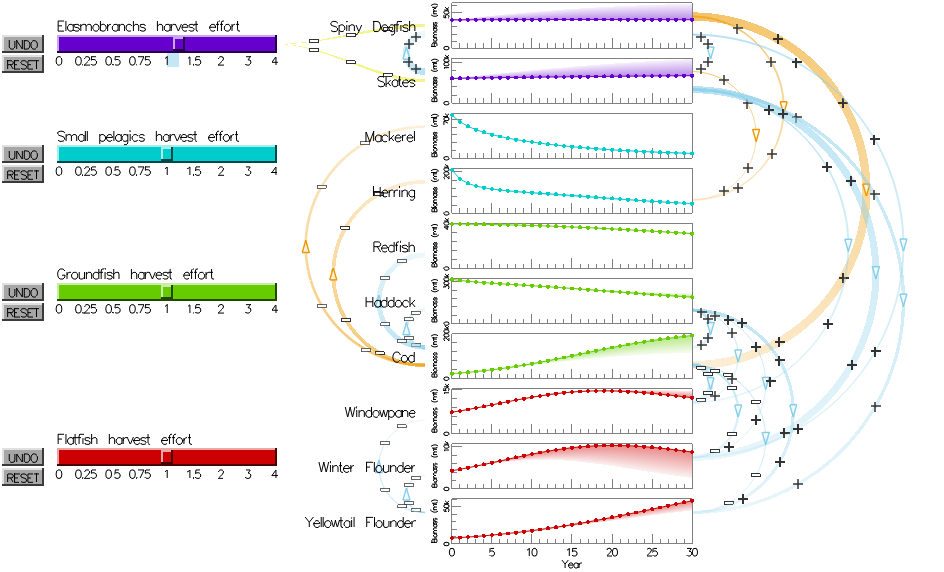
\includegraphics[width=0.98\textwidth]{figures/eps/arcs_dynamic.eps}
	\caption{Dynamic arcs drawn as a result of slightly increasing the fishing effort on elasmobranchs.}
	\label{fig:arcs_dynamic}
\end{figure}

Again, Figure~\ref{fig:arcs_dynamic} shows dynamic arcs which resulted from slightly increasing the fishing effort on elasmobranchs from 1.0 to about 1.25.  The spiny dogfish and skate biomasses both decreased as a result of the increase in fishing, as is indicated by the shaded area between the baseline forecast and the current forecast.  This is good from the perspective of all of the fish that either spiny dogfish or elasmobranchs predate on or compete with, therefore all of the arcs drawn from these two species show plus sign glyphs.  For example, spiny dogfish predate on cod, the arc between them has plus signs, and the cod biomass increased.  There are also indirect effects that the arcs help to explain.  Cod competes with windowpane, so minus signs are drawn on the arc from cod to windowpane, which helps to explain the slight decrease in the windowpane biomass.

We have realized it is possible for dynamic arcs to be misinterpreted.  Users may incorrectly assume that that absence of an arc indicates that the relationship is no longer present---e.g., if the predation arc from spiny dogfish to cod is not present, then the spiny dogfish are not eating the cod.  However, we believe that users will understand the true meaning of the arcs after a brief explanation---e.g., the arc between spiny dogfish and cod is no longer being drawn because there are no changes in the cod population that might be explained by the spiny dogfish.  When informally showing the model to users during and after development, we found that users properly interpreted the arcs after a demonstration or interaction with the model.  Another possible criticism of the dynamic arcs is that sometimes many arcs are drawn and it can become cluttered, such as when several sliders are pulled to the extremes.  However, generally less arcs are drawn in dynamic mode than static mode even in extreme cases.  Also, fishery managers may potentially be more interested in comparing the long-term effects of slight adjustments to fishing quota than dramatic adjustments that either eliminate fishing completely or wipe out entire stocks through overfishing.

\paragraph{Dynamic with Animation}

\begin{figure}[h]
	\centering
	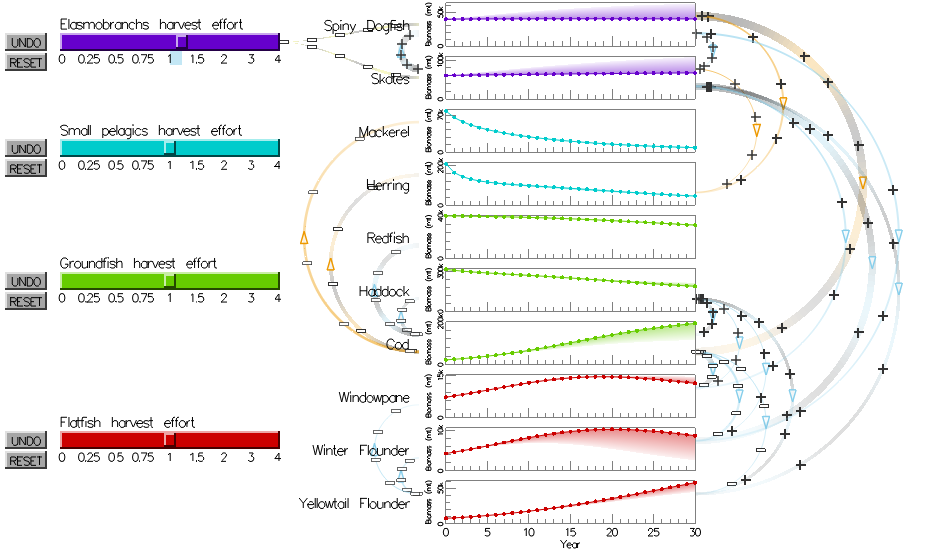
\includegraphics[width=0.98\textwidth]{figures/eps/arcs_dynamic_animated.eps}
	\caption{The same scenario as in Figure~\ref{fig:arcs_dynamic}, though with animated dynamic arc.}
	\label{fig:arcs_dynamic_animated}
\end{figure}

The third and final type for viewing the inter-species arcs is dynamic arcs with animation, seen in Figure~\ref{fig:arcs_dynamic_animated}.  In this mode, the rules for the appearance of arcs and their width is the same as in the non-animated dynamic version.  However, the plus ($+$) or minus ($-$) sign glyphs travel along the arc from the source species to the recipient species.  Additionally, the color of the arc alternates between gray and either blue, for competition, or orange, for predation.  The alteration in color also moves from source to recipient.  Both of these cues help to highlight the directionality of the arc.

\subsection{Harvest Influences}

The other type of relationship that must be ellucidated by our visualization is the harvest relationship.  While it is clear what the harvest effort value is for a particular slider, it could perhaps be clearer which species where directly affected by the harvest and how.  Therefore, we decided to draw a link is between a harvest type and a fish species, which corresponds to a fishing effort slider and a biomass small multiple, respectively, in our interface.  These links are drawn using Hermite spline curves which are colored yellow.  There are three styles for determining the width of these spline curves, which correspond to the styles for inter-species arcs: static, dynamic, and dynamic with animation.  The controls for setting the inter-species arc style also set the harvest spline curve style.  Harvest spline curves are drawn in the small multiples view whenever any type of arc is drawn.

\subsubsection{Static}

\begin{figure}[h]
	\centering
	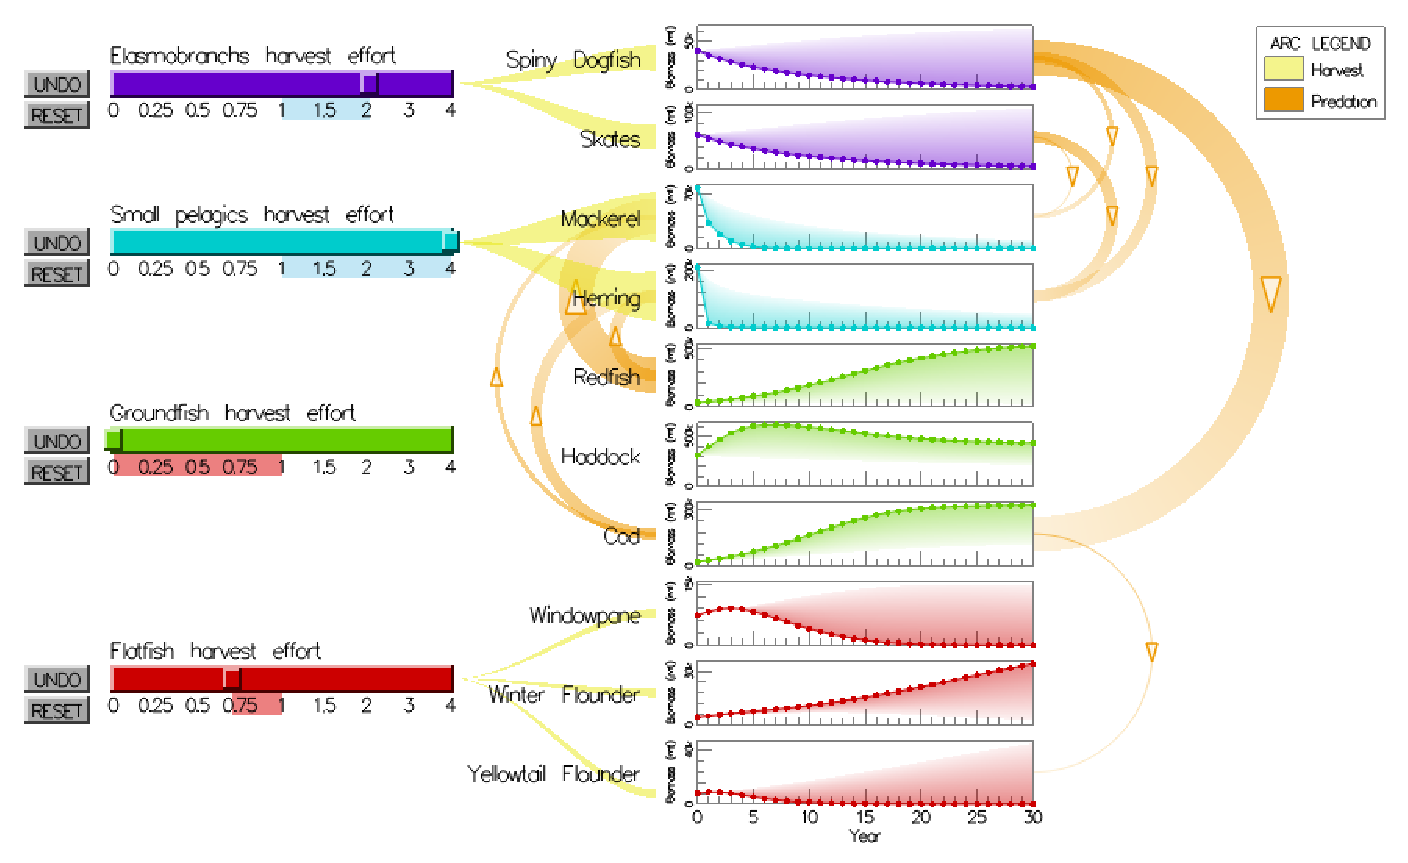
\includegraphics[width=0.98\textwidth]{figures/eps/harvest_splines.eps}
	\caption{Static harvest spline curves in yellow between effort sliders and the small multiples.}
	\label{fig:harvest_splines}
\end{figure}

In static mode, the harvest spline curve's width is directly proportional to the current value of the harvest slider, as in Figure~\ref{fig:harvest_splines}.  Therefore, when harvest effort for a specific functional group is set to zero (as it is for ``Groundfish''), then no harvest spline curves are drawn emerging from that harvest effort slider.  Likewise, the spline curves are their thickest when the matching effort slider is set to the maximum value of four (as it is for ``Small pelagics'').

\subsubsection{Dynamic}

Dynamic harvest splines can be seen in Figure~\ref{fig:arcs_dynamic}.  The width of a harvest spline in dynamic mode is proportional to the difference between the current value of the effort slider and the baseline value of the effort slider.  In other words, the width depends on a weight $w$:

\begin{align}
w = E - E'
\end{align}
where $E$ is the current effort and $E'$ is the baseline effort value for the functional group.  This is to help highlight and explain the differences between the baseline and current forecasts.   Therefore, when the harvest effort for a functional group has not been changed from the baseline, $w$ is zero and no harvest splines are drawn from that functional group's slider.

When $E' > E$ (i.e., when the harvest effort slider has been decreased), $w$ is negative.  Therefore, as with dynamic arcs for the inter-species relationships, the harvest splines have signage, which we interpreted from the perspective of the recipient, the fish being harvested.  Thus, when $w$ is negative, black plus sign ($+$) glyphs are drawn along the spline.  Conversely, when $w$ is postive, white minus sign ($-$) glyphs are drawn along the spline.  From the perspective of the fish, it is ``bad'' to be fished more and ``good'' to be fished less.  The meaning and design of these glyphs are the same as for the inter-species arcs.

\subsubsection{Dynamic with Animated}

Dynamic harvest spline curves, as in Figure~\ref{fig:arcs_dynamic_animated}, are drawn following the rules for non-animated spline curves, though with animation added.  The animation is similar to the animation for inter-species arcs:  the sign glyphs travel from the harvest effort slider to the species biomass small multiple chart and the color is alternated with gray to create a pulsing effect.  The intent was to give a clearer indication of the direction of the causal relationship.

\section{Visualization of Uncertainty}

\begin{figure}
\centering
	\begin{subfigure}[b]{0.45\textwidth}
		\centering
		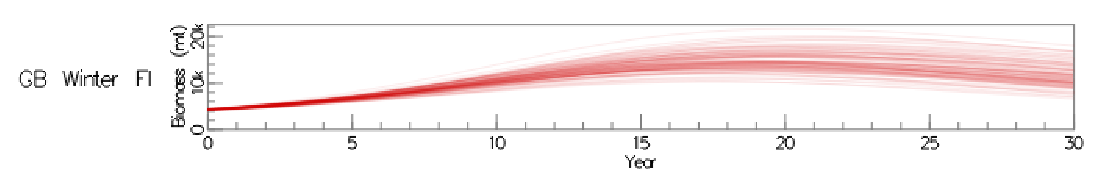
\includegraphics[width=6.5cm]{figures/eps/msprod_uncertainty_multline.eps}
		\caption{Multi-line.}
		\label{fig:uncertaintyStreak}
	\end{subfigure}	
	\begin{subfigure}[b]{0.45\textwidth}
		\centering
		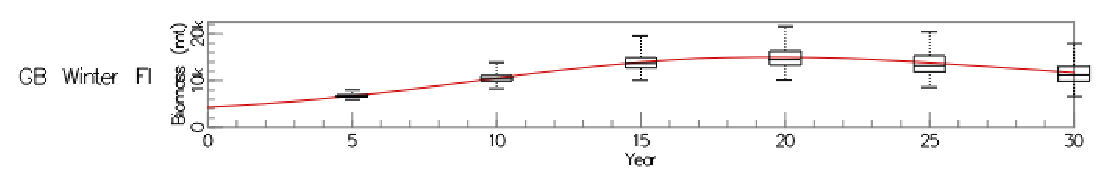
\includegraphics[width=6.5cm]{figures/eps/msprod_uncertainty_boxplots.eps}
		\caption{Box plots.}
		\label{fig:uncertaintyBoxplots}
	\end{subfigure} \\
	\begin{subfigure}[b]{0.45\textwidth}
		\centering
		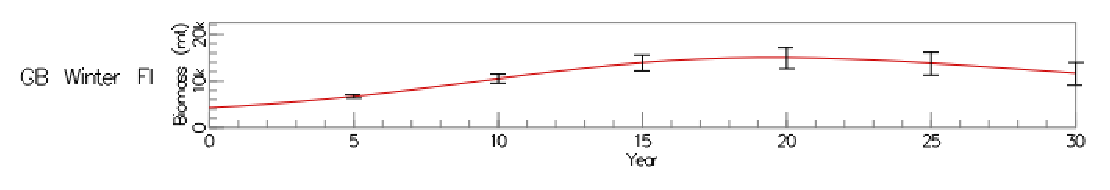
\includegraphics[width=6.5cm]{figures/eps/msprod_uncertainty_errorbar.eps}
		\caption{Error bars.}
		\label{fig:uncertaintyErrorbars}
	\end{subfigure}
	\begin{subfigure}[b]{0.45\textwidth}
		\centering
		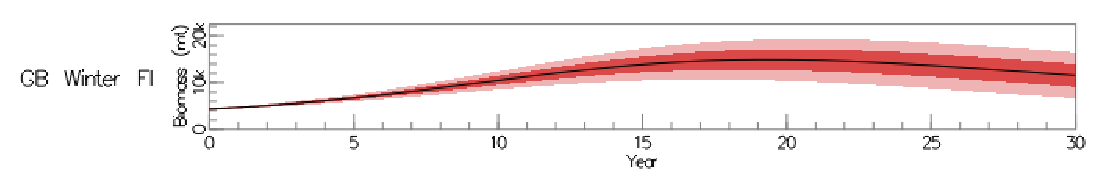
\includegraphics[width=6.5cm]{figures/eps/msprod_uncertainty_errorbands.eps}
		\caption{Error bands.}
		\label{fig:uncertaintyErrorbands}
	\end{subfigure}
	\caption{The four methods for visualizing uncertainty of MS-PROD model simulations.}
	\label{fig:uncertainty}
\end{figure}

Since models are simplifications of reality, their output is best understood as a range of expected values.  It is possible that a representation of uncertainty may aid decision making.  To add uncertainty visualization to the MS-PROD model, our interface can perform Monte Carlo simulations by jittering the non-zero input parameter values $\pm 10\%$ with a normal distribution.

The resulting uncertainty can be displayed in four styles.  First, a multi-line option shows the uncertainty by drawing one semi-transparent line for each run of the Monte Carlo simulation, as in Figure~\ref{fig:uncertaintyStreak}. This was inspired by Cox et al.'s new method for displaying hurricane tracks \cite{cox2013}.  The second option displays a traditional box plot every five years, as in Figure~\ref{fig:uncertaintyBoxplots}.  Third, in Figure~\ref{fig:uncertaintyErrorbars}, a summary line is drawn, with bars every five years.  Lastly, Figure~\ref{fig:uncertaintyErrorbands} shows a summary line in solid black line with bands.

In all options but the multi-line option, the user has the ability to display different statistical data in the selected style.  Users can select between mean and median for the ``summary'' lines.  Box plots, error bars, and error bands can represent either quartiles with minimum and maximum data values or two standard deviations.  This allows the user to easily explore the distribution of data under different representation with a few clicks of the mouse.  The multi-line option may appeal to less scientific users, while the other more traditional representations of statistical data may appeal to advanced users, such as modelers or fishery managers, but all users have all options at their disposal.

%to indicate the boundaries of the first, second (median), and third quartiles with whiskers stretching to the minimum and maximum values
% mean of all simulations is displayed as a line
